\chapter{Data models and transformations}

The data about the academic researchers and their publications at \ac{CUNI} is internally stored in a relational database. 
The first chapter of this thesis explores the transformation of the relational data model into a graph data model, 
which will allow us to use the graph algorithms for the social network analysis.

We also address pitfalls and challenges of the transformation stemming 
from the specific nature of the data and the technical limitations of the source systems.

\section{Input data format}

The Charles University information system is composed of a set of separate systems and applications.

The \textit{Studium} information system\footnote{Available at \url{https://is.cuni.cz/studium/}.} contains the data about the researchers, teachers, the courses and study programmes available at the university.

The \textit{Věda} information system\footnote{Available at \url{https://is.cuni.cz/veda/}, login only.} aggregates the data about creative activities of the researchers, the research projects and inter-university mobility programmes.
For the purpose of this thesis, we are mostly interested in the \ac{OBD} (or Verso) module, containing the data about the academic publications.

The \textit{Whois} staff information system\footnote{Available at \url{https://is.cuni.cz/webapps/whois2}.} contains the data about the employees of the university, 
their affiliations with the faculties and departments and their academic titles.

While none of the systems offer public APIs, a data import pipeline has been set up by \ac{ÚVT} (the university's IT department) in advance
for the purpose of the Charles Explorer application. 
This pipeline consists of a set of database views tracking the changes in the data and a script\footnote{\url{https://gitlab.mff.cuni.cz/barj/charles-explorer/-/blob/master/scripts/export.sh}} that exports the data to an SQLite database.


\section{Target data model}\label{sec:target-data-model}

We aim to transform the relational data model into a graph data model, which will allow us to use the graph algorithms for the social network analysis.

While the available data would allow us to create a multi-relational graph model with different types of nodes and edges (e.g. \textit{Person}, \textit{Publication}, \textit{Course}, \textit{Study programme}), 
we limit the scope of this thesis to the social network between the \textbf{academic researchers} and their \textbf{publications}.

From the view of the input data, this is the largest and most interconnected part of the data, which will allow us to demonstrate the capabilities of the graph algorithms.
The connections in the resulting graph are also easily interpretable (e.g. the co-authorship relations between the researchers, the authorship relations between the researchers and the publications).

The nodes of the graph will represent the academic researchers and the publications, while the edges will represent the co-authorship relations between the researchers and the authorship relations between the researchers and the publications.

We can notice that the graph is a \textit{bipartite graph}, as the nodes can be divided into two disjoint sets - the set of the researchers and the set of the publications.

\subsection{Exploring the schema}

To illustrate the structure of the input data, we provide an example of the schema of the relational database together with example data.
Since this thesis focuses on the social network between the academic researchers and their publications, we limit this example only on the relevant parts of the schema.

The social network-relevant data accessible in the following three database views:

\begin{Verbatim}[commandchars=\\\{\}]
PERSON (
    \verbun{\verbbf{PERSON_ID}}, \verbxs{- \ac{UKČO} personal number}
    PERSON_NAME, \verbxs{- Full name of the person, incl. the academic titles}
    PERSON_WEBSITE, \verbxs{- Personal website of the person}
    \verbun{\verbbf{PERSON_WHOIS_ID}}, \verbxs{- ID of the person in the Whois system}
    TYPE \verbxs{- Person type - teacher(U), external employee(E), or other(O)}
)
\end{Verbatim}

The \texttt{Person} view contains the data about the academic researchers and teachers at the university.
While the \texttt{TYPE} column might suggest that the table contains records about external people as well (e.g. guest co-authors of publications published by the \ac{CUNI} researchers),
it only contains the data about the people affiliated with the university. The \texttt{TYPE} column is only used to distinguish between the different employment types at the university.

\begin{Verbatim}[commandchars=\\\{\}]
PUBLICATION_KEYWORDS (
    \verbun{\verbbf{PUBLICATION_ID}}, \verbxs{- internal ID of the publication}
    PUB_YEAR, \verbxs{- year of the publication}
    TITLE, \verbxs{- title of the publication}
    ABSTRACT, \verbxs{- abstract of the publication}
    KEYWORDS, \verbxs{- keywords of the publication}
    LANGUAGUE\verbxs{(sic!)}, \verbxs{- ISO 639-2 language code of the TITLE,}
                              \verbxs{ABSTRACT and KEYWORD columns}
    ORIGINAL\verbxs{ - whether the LANGUAGUE column is the original}
                               \verbxs{language of the publication}
)
\end{Verbatim}

This schema shows some more issues with the data - the \texttt{PUBLICATION\_KEYWORDS} is missing a single primary key attribute,
as the \texttt{PUBLICATION\_ID} is not unique across the table. This is because the same publication can have multiple records in the table,
each record representing a different language version of the title, abstract and keywords.

Moreover, the \texttt{PUBLICATION\_KEYWORDS} view does not contain an universally accepted publication identifier (e.g. a \ac{DOI} or an \ac{ISBN}) 
that would allow us to link the publication to the external sources of the publication data.
This is because of a technical limitation of the information systems, as the \ac{OBD} module is not fully interoperable with the \textit{Studium} module we are 
consuming the data from.

\label{sec:pub-author-all}
\begin{Verbatim}[commandchars=\\\{\}]
PUBLICATION_AUTHOR_ALL (
    \verbun{PUBLICATION_ID}, \verbxs{- internal ID of the publication}
    \verbun{PERSON_ID}, \verbxs{- \ac{UKČO} personal number of the author, if available}
    PERSON_NAME, \verbxs{- Full name of the author, incl. the academic titles}
)
\end{Verbatim}

The relational database view \texttt{PUBLICATION\_AUTHOR\_ALL} contains the links between the publications and the authors from the previous views.

With the most naive approach, the transformation of the relational data model into a graph data model could be done by transforming the records of the 
\texttt{PERSON} and (deduplicated) \texttt{PUBLICATION\_KEYWORDS} views into the nodes of the graph, 
and the records of the \texttt{PUBLICATION\_AUTHOR\_ALL} view into the edges of the graph.

\section{Inferring missing identities}\label{sec:inferring-missing-identities}

    In the \hyperref[sec:pub-author-all]{comment} for the \texttt{PUBLICATION\_AUTHOR\_ALL.PERSON\_ID} column, we note that the \ac{UKČO} personal number is not always available.
    This is because of external authors, who are not affiliated with the university and do not have a \ac{UKČO} personal number.
What is worse, such authors are only identified by their name and academic titles, which can be inconsistent across the publications.
This is again caused by the limited interoperability of the \ac{OBD} and \textit{Studium} modules.

Aside from the obvious implications of this issue - i.e. user confusion and potential performance issues,
this also poses a challenge for the social network analysis, as the graph algorithms might not be able 
to correctly identify the external authors.

    In the aforementioned \texttt{PUBLICATION\_AUTHOR\_ALL} view, counts of the relations mentioning the authors with / without the \ac{UKČO} personal number are as follows:

\begin{figure}[!ht]
    \captionsetup{width=.9\linewidth}
    \centering
    \begin{tabular}{|c|c|c|}
    \hline
        Type & Count & Distinct \\ \hline
        PERSON\_ID present & 808467 & 39523 \\ \hline
        PERSON\_ID missing & 671332 & ? \\ \hline
    \end{tabular}
    \caption{Counts of the relations in the \texttt{PUBLICATION\_AUTHOR\_ALL} view.}
\end{figure}

We see that the no-identifier authors take up to 45\% of the total count of the relations.
This explains the importance of the problem of inferring the missing identities.

\subsection{Naïve approach}\label{sec:naive-approach}

The naïve solution to this problem is using the \textit{names} for the identity inference 
in case of missing identifiers.
While this is a simple and straightforward transformation, it has obvious drawbacks.

Firstly, the names are not guaranteed to be \textit{unique} across the dataset. 

Secondly, the names are not guaranteed to be \textit{consistent} across the dataset - due to (e.g. marital) name changes, 
typos, or different conventions in the academic titles.
See the example of a search for the name ``Jaroslav Peška'' in the \texttt{PUBLICATION\_AUTHOR\_ALL} view:

\begin{figure}[!ht]\label{fig:jaroslav-peska}
    \captionsetup{width=.9\linewidth}
    \centering
    \begin{tabular}{|c|c|c|}
    \hline
        COUNT(*) & PERSON\_NAME & PERSON\_ID \\ \hline
        2 & doc. PhDr. Jaroslav Peška Ph.D. & 14124313\dots \footnotemark \\ \hline
        5 & doc. PhDr. Jaroslav Peška Ph.D. & null \\ \hline
        2 & Doc. PhDr. Jaroslav Peška Ph.D. & null \\ \hline
        1 & doc. PhDr. Jaroslav Peška PhD. & null \\ \hline
        4 & Jaroslav Peška & null \\ \hline
    \end{tabular}
    \caption{Search for the name ``Jaroslav Peška'' in the \texttt{PUBLICATION\_AUTHOR\_ALL} view.}
\end{figure}

\footnotetext{PERSON\_ID redacted for privacy reasons, replaced by truncated PERSON\_WHOIS\_ID.}

    While there are 5 variants of the same name in the dataset, only one of them is correctly linked to the \ac{UKČO} personal number.
This could have been caused by human error on data input or by the limitations of the source systems. 
Either way, this creates an unrecoverable loss of information in the dataset.

In the SQL database export, we can ``merge'' the records using the naïve approach efficiently using a many-to-one (non-injective) mapping
on the \texttt{PERSON\_NAME} column.

Let us define a function $f$:
$$f: \text{PERSON\_NAME} \to \text{NORMALIZED\_NAME}$$

We require $f$ to map all person names to a \textit{normalized form}, which is defined as follows:
\begin{itemize}
    \item The academic titles are stripped from the name.
    \item The name is converted to lowercase.
    \item The name is stripped of any diacritics.
    \item The name is stripped of any non-alphabetic characters.
    \item The whitespace characters are normalized to a single space.
    \item The name is stripped of any leading or trailing whitespace.
\end{itemize}

We can see that in the case of \hyperref[fig:jaroslav-peska]{Jaroslav Peška}, 
the normalized version for all the variants is the same (i.e. $f(\texttt{PERSON\_NAME}) = \texttt{jaroslav peska}$).

If we decide to add the output of this normalization function as an attribute in the \texttt{PUBLICATION\_AUTHOR\_ALL} view,
we can proceed with the merging of the records using SQL GROUP BY and the aggregation functions.

% \label{infobox:sqlite-loadable-extensions}
\begin{mybox}
    {SQLite Loadable Extensions}

    While it would be possible to implement the normalization function using inbuilt scalar SQLite functions (namely \texttt{lower}, \texttt{trim},
    and repeated use of \texttt{replace}), the developer experience of such solution is suboptimal, as it requires a lot of nested function calls
    in the \texttt{SELECT} clause.

    Because the way the scalar functions are defined in SQLite - and their implementation\footnote{\url{https://sqlite.org/src/file?name=src/func.c}}, 
    the repeated calls to \texttt{replace} also result in repeated string allocations and deallocations - which can be a performance bottleneck.

    Fortunately, SQLite allows the user to define their own loadable extensions\footnote{\url{https://www.sqlite.org/loadext.html}} in C.
    This allows us to define the normalization function in C and load it as a scalar function in the SQLite database.
\end{mybox}

\textbf{Implementation}

For the implemetation of the name normalization function, we use the SQLite loadable extensions mechanism.
The transformation itself is done in three steps:

\begin{enumerate}
    \item Using the \texttt{glib} function \texttt{g\_utf8\_normalize}, the string representation of the name is normalized to the canonical Unicode \ac{NFD} form.
    This step ensures that the byte representation of diacritized characters is now composed of separate characters for the base character and the diacritics (e.g. \texttt{ě}\texttt{(U+011B)} is decomposed to \texttt{e}\texttt{(U+0065)} and \texttt{ˇ}\texttt{(U+02C7)}).
    \item We scan the normalized string and remove all the characters that are not in the range of the Latin alphabet. We convert the all the 
    alphabetic characters to lowercase and replace all the whitespace characters with a single space.
    \item Using regular expressions, we remove the academic titles from the name. 
    We construct the expression by defining a list of the academic titles and concatenating them using the alternative separator \texttt{|} (e.g. \texttt{PhDr.|Ph.D.}).
    We then use this regex to find the start index of the actual person name in the string
    and use the \texttt{glib} function \texttt{g\_strndup} to extract the substring.
\end{enumerate}

The full implementation of the normalization function is available in the GitHub repository of this thesis.\footnote{\url{https://github.com/barjin/master-thesis/tree/main/examples/sqlite-normalize-ext}}.

For reference purposes, we also implement the same normalization function using Python.
This implementation loads the data from the database, normalizes the names using a Python function, and writes the normalized names into a new table.
The implementation can also be found in the GitHub repository\footnote{\url{https://github.com/barjin/master-thesis/tree/main/examples/sqlite-normalize-python}}.

\textbf{Performance}

As mentioned in the infobox above, the SQLite extension for normalizing the names should provide a performance improvement over the composed scalar functions.
To test this hypothesis, we repeatedly construct a temporary table with the normalized names using the both scalar functions and the extension.

\begin{figure}[!ht]
\begin{verbatim}
CREATE TABLE test AS 
    SELECT normalize_name(PERSON_NAME) -- or the scalar functions
        AS NORMALIZED 
    FROM PUBLICATION_AUTHOR_ALL;
\end{verbatim}
\captionsetup{width=.9\linewidth}
\caption{The SQL query for the performance test of different normalization methods.}

\end{figure}

SQLite engine has a default limit on the maximum expression tree depth of 1000\footnote{\url{https://www.sqlite.org/limits.html\#max_expr_depth}}.
This limit is quite low and can be easily reached when using the composed scalar functions.

Because of this limitation, we are not replacing all of the academic titles in the \textit{composed scalar functions} case of the experiment.
Even with the reduced number of operations, the composed scalar functions seem to be much slower than the SQLite extension:

\begin{figure}[ht!]
    \captionsetup{width=.9\linewidth}
    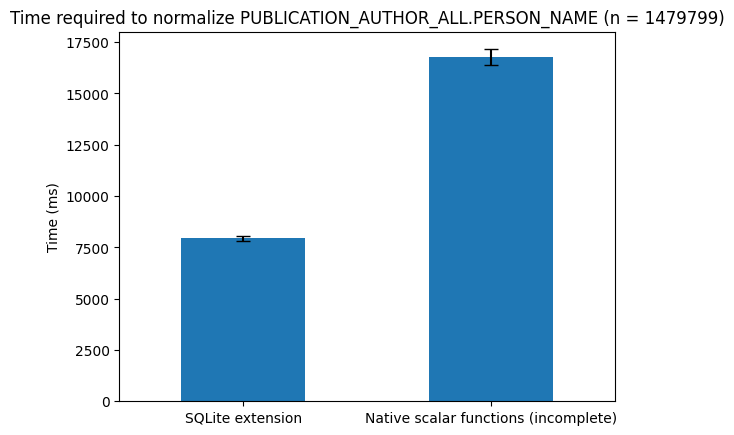
\includegraphics[width=\textwidth]{../img/sqlite_vs_native_scalar_functions.png}
    \centering
    \caption{The performance comparison of the SQLite extension and the composed scalar functions (mean over 10 runs).}
\end{figure}

The Python reference implementation is expectedly much slower than both the SQLite extension and the composed scalar functions.
This is likely caused by the interface read-write overhead of the Python \texttt{sqlite3} library - as compared to the native data access of the SQLite extension.

\textbf{Results assessment}\label{sec:results-assessment}

After the normalization and aggregating the records using the normalized names,
we get \texttt{240001} distinct normalized names in the dataset.

% todo factcheck
The most frequent external author was \textit{B. Abbott} with $1393$ records, followed by $G. Aad$ with $1191$ records.
This raises concerns about the uniqueness of the normalized names - as with $1339$ coauthored publications, \textit{B. Abbott} would be the 99.9 percentile (or the top 7th author),
compared to the internal authors with known identifiers.

\textbf{Issues with the naïve approach}

While the naïve approach is simple and straightforward, it poses several issues.

Firstly, name-based merging can be problematic in the case of the authors with common names, as likely seen in the \hyperref[sec:results-assessment]{results assessment}.

Secondly, there is no support for the existing identifiers from the dataset.
By only inferring the identifier from the name, we willingly discard the existing information about the person.

This could be partially solved by coalescing the inferred identifiers with the existing ones.
Using the SQL \texttt{COALESCE} function, we can create a new column in the \texttt{PUBLICATION\_AUTHOR\_ALL} view that would contain the inferred identifier only if the original one is missing.

However, such approach would only fully work in the case of only internal - or only external authors.
In the case of the internal authors with few records with missing identifiers (e.g. \hyperref[fig:jaroslav-peska]{Jaroslav Peška}),
this would still result in the creation of up to two nodes for the same person (i.e. \texttt{14124313...} for the ``internal'' records and \texttt{jaroslav-peska} for the ``external'' ones).

\begin{mybox}{``On-demand'' naïve identity inference}

In an attempt to solve the over-merging issue of the authors with common names in the naïve approach, we slightly modify the algorithm.

Instead of merging the records directly in the database, we merge the records on-demand in the application's visualization layer.
If we e.g. restrict the direct views only to internal authors - and show the external authors only as collaborators of those,
we can reuse the naïve approach quite effectively.

By restricting the domain of the mergeable records to a smaller, tighter subcomunity of the graph (i.e. collaborators of one internal author), 
we reduce the number of the possible false positives in the merging.

Obviously, this approach still carries the risk of the false positives in case of different external authors with the same name in the same subcommunity.

Also note that this approach only improves the user experience with the application.
Using this, every external author's coauthorship is stored as a separate node in the graph, which can negatively impact the performance of the graph algorithms.
\end{mybox}


\subsection{Distance-based hierarchical clustering}

To solve the issues of the naïve approach, we can try to use the graph structure of the data to infer the missing identities.
One of the possible approaches is to use the \textit{hierarchical clustering} methods to group the nodes from similar parts of the graph together.

In the realm of data mining and statistics, \textit{hierarchical clustering} is an umbrella term for a set of unsupervised learning algorithms for grouping
given data points into a hierarchy of clusters. Typically, these algorithms iteratively merge the closest clusters together, until only one cluster remains.\footnote{In case of top-down clustering, the process is reversed.}
The distance metric used for the clustering can be any metric that defines the similarity between the data points.

\subsubsection{Algorithm}\label{sec:distance-based-hierarchical-clustering}

In the case of our dataset, we can use the shortest path distance between the nodes in the graph as the distance metric.

We define the merging process as follows:

\begin{enumerate}
    \item Start with a graph with nodes only merged based on explicit identifiers. \texttt{PUBLICATION\_AUTHOR\_ALL} records without an explicit identifier are represented as separate nodes.
    \item Select an arbitrary unmerged node without an identifier.
    \begin{enumerate}
        \item Using the \hyperref[sec:naive-approach]{naïve approach}, we find all merge candidates for the selected node. Note that we are using the normalized name equality as the requirement for the merge.
        \item We calculate the distance matrix between the selected node and all the merge candidates.
        \item Using a hierarchical clustering algorithm, we cluster the data points based on the distance matrix. We select the cut-off distance based on the distance distribution.
    \end{enumerate}
    \item Go to step 2 until all the non-identifier nodes are merged.
\end{enumerate}

We can make a few observations in the internal loop of the second step.
As mentioned in \ref{sec:target-data-model}, the graph containing the nodes with the explicit identifiers is a \textit{bipartite graph}.
Because of this, any path between two person-type nodes is even-lengthed.
Therefore, the shortest path distance between two person-type nodes is 2.

Additionally, the shortest path distance between two \textit{mergeable} nodes is 4.
This is based on an observation that two person nodes in distance 2 are connected to the same publication node.
In case there are two merge candidates (based on the naïve mergeability requirement) connected to the same publication node,
these should not be considered \textit{mergeable}, as the publication is expected to list unique authors - i.e. the candidates are
different people with the same name.

\subsubsection{Implementation}

The \hyperref[sec:distance-based-hierarchical-clustering]{proposed algorithm} 
is computationally expensive. The distance matrix calculation has a time complexity of $O(n^2)$
and the standard hierarchical agglomerative clustering algorithm has a time complexity of $O(n^3)$.

\textbf{Distance matrix calculation}

Loading the social network into Memgraph\footnote{An open-source in-memory graph database. Available at \url{https://memgraph.com/}.}
, we quite easily implement the calculation of the distance matrix between the merge candidates using the Cypher graph query language.

\begin{figure}[!ht]
\begin{verbatim}
    MATCH path=(p1: Person)-[*BFS]-(p2: Person)
    WHERE 
        p1.PERSON_ID IN $queryCandidates 
        AND p2.PERSON_ID IN $queryCandidates
        AND p1.PERSON_ID < p2.PERSON_ID
    RETURN 
        p1.PERSON_ID, 
        p2.PERSON_ID, 
        size(path) AS distance
\end{verbatim}
\captionsetup{width=.9\linewidth}
\caption{The Cypher query for the distance matrix calculation.\protect\footnotemark}
\label{fig:distance-matrix-calculation}
\end{figure}

\footnotetext{Rather curiously, passing the IDs array as a parameter results in a highly inefficient execution plan in Memgraph causing a full scan of the nodes followed by a filter on the PERSON\_ID.
Inlining the parameter array into the query causes Memgraph to use faster indexed access.}

In this query, \texttt{\$queryCandidates} is an array containing the node identifiers of the merge candidates for a given normalized name group.
Note that the query results can also be paginated using the \texttt{SKIP} and \texttt{LIMIT} clauses.

Preliminary experiments show that the query execution time is around \texttt{5.37} ms per pair of nodes.
Calculating the matrix of e.g. \texttt{490000} pairs (for an external author consisting of 700 merge candidates) would take around 43 minutes.
While this is a one-time operation - and the distances cannot change, as the external author nodes are always connected only to the one publication they are attributed to - this still leaves space for optimization.

%% todo add graphs
\begin{mybox}
    {Optimization: Monopartite projection}

    The run time of the distance matrix calculation is artificially increased by the \textit{bipartitedness} of the graph.
    During the calculation of the shortest path distance between two person nodes, 
    the breadth-first search algorithm is forced to explore the intermediate publication nodes - even though those have no possibility of being the target node.
    This can inflate the size of the internal BFS queue and the number of the visited nodes.
    
    To mitigate this issue, we can calculate the distance matrix in \texttt{2(b)} on the \hyperref[def:monopartite-projection]{monopartite projection} of the social network on 
    the set of the \textit{person nodes}. By replacing the publication nodes with edges on the person nodes, we reduce the lengths of the shortest paths in half.
\end{mybox}

While the monopartite projection of the social network can be calculated using the Cypher query language in Memgraph,
we transform the data straight in the source SQL database. Using a self \texttt{INNER JOIN} on the \texttt{PUBLICATION\_AUTHOR\_ALL} view over the \texttt{PUBLICATION\_ID} column,
we receive the monopartite projection of the social network on the set of the person nodes. Projecting the data onto the person identifiers
leaves us with a table containing the pairs of the person identifiers connected by an edge.

\begin{figure}[!ht]
\begin{verbatim}
SELECT DISTINCT X.PERSON_ID, Y.PERSON_ID 
   FROM (
      SELECT PERSON_ID, PUBLICATION_ID FROM PUBLICATION_AUTHOR_ALL
   ) AS X 
   INNER JOIN (
      SELECT PERSON_ID, PUBLICATION_ID FROM PUBLICATION_AUTHOR_ALL
   ) AS Y 
USING(PUBLICATION_ID)
WHERE X.PERSON_ID < Y.PERSON_ID;
\end{verbatim}
\captionsetup{width=.9\linewidth}
\caption{The SQL query calculating the monopartite projection of the social network.}
\label{fig:monopartite-projection}
\end{figure}

Note that the \texttt{PERSON\_ID} in the query above is either the internal person identifier or a \textit{generated unique identifier} for the external authors.

Unfortunately, even with the projected graph, the performance of the shortest path distance calculation in Memgraph is still suboptimal. 
With the mean time of \texttt{5.68} ms per pair of nodes, this approach does not provide any significant performance improvement over the original one.

This might be caused by the specific structure of the academic social network, where the person nodes are connected by a much small number of publication nodes.
This is especially true with the graph with external authors, where the external author nodes are connected only to the one publication node.

Note that the BFS algorithm has complexity of $\mathcal{O}(V + E)$, where $V$ is the number of the nodes and $E$ is the number of the edges.
While the monopartite projection reduces the number of the nodes in the graph, it does not reduce the number of the edges - as the publication nodes are replaced 
by the edges between the all the coauthoring person nodes. 

In case of the process described with the \hyperref[fig:monopartite-projection]{Figure 2.6}, each publication node is replaces 
by $k$ edges, where 
$$
k = \binom{deg(v)}{2}
$$

for $deg(v)$ being the \hyperref[def:node-degree]{degree} of the publication node $v$.

\newpage

\begin{mybox}
    {Optimization: BFS ``vectorization''}

    Memgraph resolves the \hyperref[fig:distance-matrix-calculation]{Cypher query} for calculating the distance matrix
    with execution plan that includes a shortest path operation for \textit{each node pair}.

    While Memgraph uses a slightly optimized algorithm\footnote{Expanding the BFS fringe from both ends (\href{https://github.com/memgraph/memgraph/blob/58c3902c194e80a027d141788bd1afd07def0114/src/query/plan/operator.cpp\#L1569-L1572}{see source on GitHub}).} for calculating the shortest path distance between the two nodes,    
    the distance matrix calculation can still be optimized by using a \textit{vectorized} approach.

    During a regular BFS, the algorithm visits growing $k$-hop neighborhoods of the start node until it finds the target node.
    Since in our case, we are calculating the entire distance matrix (for a set of nodes), 
    we can optimize the process by searching for all the target nodes in the same BFS run.
    This allows us to acquire the shortest path distances between the start node and all 
    the target nodes in a single BFS run.

\end{mybox}

The algorithm itself is quite simple and differs from the regular BFS approach only in several details.
The following pseudocode example describes the vectorized BFS algorithm:

\begin{algorithmic}[1]
    \Function{VectorizedBFS}{graph, start, targets}
        \State $visited, queue, distances \gets \emptyset$
        \State $queue.\text{push}(start, 0)$
        \While{$\text{not } queue.\text{empty}() \text{ and } \underline{\textbf{not } targets.\text{empty}()}$}
            \State $(node, depth) \gets queue.\text{pop}()$
            \If{$node \text{ in } targets$}
                \State $distances[node] \gets depth$
                \State $\underline{targets.\text{remove}(node)}$
            \EndIf
            \For{$neighbor \text{ in } graph[node]$}
                \If{$neighbor \text{ not in } visited$}
                    \State $queue.\text{push}((neighbor, depth + 1))$
                    \State $visited.\text{add}(neighbor)$
                \EndIf
            \EndFor
        \EndWhile
        \State \Return $distances$
    \EndFunction
\end{algorithmic}

Notice the underlined parts of the algorithm - these are the parts that differ from the regular breadth-first search for a single target node.
Unlike the single target BFS, the vectorized version only terminates once all the target nodes are visited.

Note that - given we consider the \textit{targets} list constant-sized - the algorithm has the same asymptotic complexity as the regular BFS - i.e. $\mathcal{O}(V + E)$.
This is obvious if we compare this vectorized approach to the regular single-target BFS for the \textit{furthest} target node.
Both algorithms visit the same number of nodes and edges, the only difference is in the output - the vectorized BFS outputs the distances to all the target nodes.

At the time of writing this thesis (\today), the vectorized BFS algorithm is not implemented
in Memgraph or any other major graph database (Neo4j, OrientDB, ArangoDB). 
While with the vertex identifiers inlined in the query, the Cypher query planner might be able to automatically recognize the 
need for the vectorized BFS, the obscure nature of the use case is likely the reason for the lack of the implementation.

Because of this, we implement our own distance matrix calculator based on the vectorized BFS algorithm in C++\footnote{Implementation at \url{https://github.com/barjin/master-thesis/tree/main/examples/distance-matrix}}.
This program takes the graph data - i.e. the output of \hyperref[fig:monopartite-projection]{Figure \ref*{fig:monopartite-projection}} - in CSV format and parses the data into an in-memory graph representation.
It then iterates over a list of the user-specified target nodes, taking each node as the start node for the \textit{VectorizedBFS} algorithm.
The rest of the list is used as the target nodes for the algorithm. 

By iterating through the list of the target nodes, we calculate the distance matrix in $k$ BFS runs, where $k$ is the number of the target nodes.
This is a significant improvement over the $k^2$ BFS runs in the original Memgraph approach.

\begin{figure}[ht!]
    \captionsetup{width=.9\linewidth}
    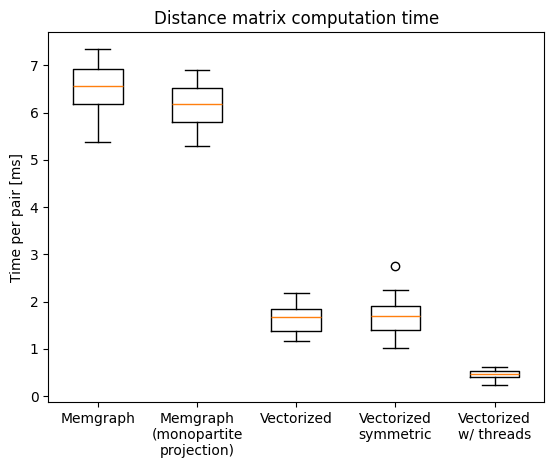
\includegraphics[width=0.7\textwidth]{../img/identity_inferrence_distance_matrix.png}
    \centering
    \caption{The performance comparison of different distance matrix calculation methods.}
    \label{fig:identity-inferrence-benchmarks}
\end{figure}

Benchmarks show that the vectorized BFS algorithm is with mean time of $1.65\text{ ms}$ per pair of nodes significantly faster than the regular BFS algorithm.

\hyperref[fig:identity-inferrence-benchmarks]{Figure \ref*{fig:identity-inferrence-benchmarks}} compares the results to two more possible optimizations of the vectorized approach.

The \textbf{Vectorized symmetric} approach only calculates the upper triangle of the distance matrix and mirrors the results to the lower triangle.
This utilizes the fact that the social network graph we are using is undirected - i.e. the shortest path distance between the nodes $u$ and $v$ is the same as the distance between the nodes $v$ and $u$.
This makes the distance matrix symmetric, and allows us to save half of the calculations by only calculating the upper triangle.

This approach brings next to no performance improvement over the regular vectorized BFS.
The reason becomes apparent when we consider the fact that the vectorized BFS's complexity is $\mathcal{O}(V + E)$ - i.e. does not depend on the number of the target nodes.

The approach labeled \textbf{Vectorized w/ threads} parallelizes the vectorized BFS algorithm using multithreading.
Since the BFS algorithm is inherently sequential, the parallelization is done on the outer loop iterating through the start nodes.
The parallelization itself is quite straightforward, as \textit{VectorizedBFS} is a pure function with no side effects.

This approach comes out as the most performant, with the mean time of $0.45\text{ ms}$ per pair of nodes.

\textbf{Hierarchical clustering}

After calculating the distance matrix, we can proceed with the hierarchical clustering algorithm.
For the purpose of this thesis, we will be using specifically the bottom-up agglomerative clustering algorithm.

The Python library \texttt{scipy} provides an implementation of the hierarchical clustering algorithm in the \texttt{scipy.cluster.hierarchy} module.
Applying this algorithm to the distance matrices calculated in the previous step, we can cluster the nodes based on the distance matrix.
